\section{Estimación de Pose en Humanos}

%  https://nanonets.com/blog/human-pose-estimation-2d-guide/
%  https://viso.ai/deep-learning/pose-estimation-ultimate-overview/
%  https://arxiv.org/pdf/2012.13392.pdf
%  https://sci-hub.se/10.1016/j.cviu.2019.102897
%  https://sci-hub.se/10.1109/access.2020.3010248
%  https://sci-hub.se/10.1016/j.cviu.2016.09.002
%  https://stasiuk.medium.com/pose-estimation-metrics-844c07ba0a78

La tarea de \textit{Estimación de Pose en Humanos} (HPE por sis siglas en inglés) ha sido uno de los
tópicos de gran importancia en
el campo de Visión por Computadora. Debido a la búsqueda de automatización y entendimiento de
diversas actividades humanas, sus utilidades causan impacto directo en las implementaciones
tecnológicas del mundo real, tales como, la predicción de intención (vigilancia), sistemas de
autónomos y de asistencia en la conducción automóviles, animación, simulaciones,
interacción Humano-Computadora (HCI), realidad virtual
aumentada (VR y AR), videojuegos, salud o asistencia médica o hasta análisis de movimiento en
deportes. La tarea de \textit{Estimación de Pose} no solo se limita a el cuerpo
humano, también, puede ser empleado en objetos como carros o animales, vease la imagen \ref{fig:PE-track}.

Con el crecimiento acelerado de \textit{Aprendizaje Profundo} en los últimos años gracias a las
capacidades actuales de potencia de cómputo los métodos basados bajo este enfoque han sobrepasado
a las métodos tradicionales, sin embargo aún existen distintos problemas y retos que siguen presentes
como la oclusión y la ambiguedad de los datos o la dificultad de su obtención para realizar
entrenamientos.

\begin{figure}[ht!]
    \centering
    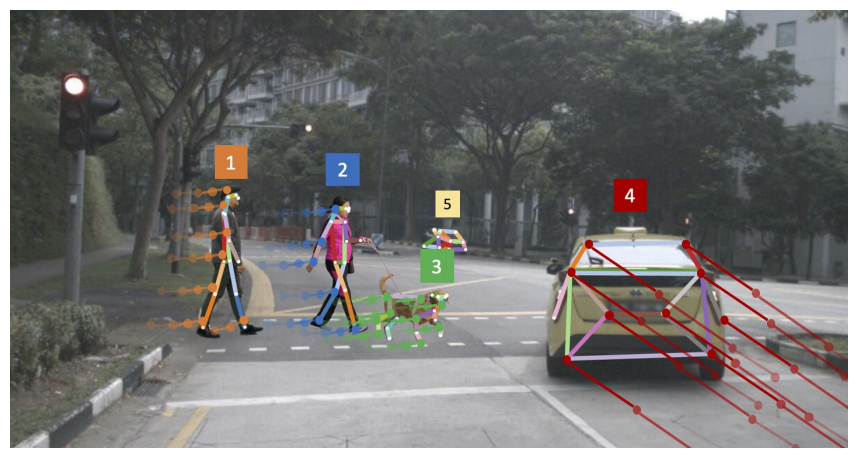
\includegraphics[width=0.4 \textwidth]{Chapters/1. HPE_LUNG/figures/openpifpaf.png}
    \caption{OpenPifPaf: Escena del mundo real desde la perspectiva de un carro autónomo. Todos los
             actores son detectados y seguidos, esto incluye a las personas, el carro y el perro.
             \cite{DBLP:journals/corr/abs-2103-02440}}
    \label{fig:PE-track}
\end{figure}

El problema de \textit{Estimación de Pose Humanos} consiste en predecir las partes del cuerpo o las
posiciones de las articulaciones de una persona a través de una imagen, video. Este problema ha sido
cuidadosamente estudiado a lo largo de los años y diversas recopilaciones de investigaciones han sido escritas.
En la tabla \ref{Tab:hpe-survey} se resumen algunas de las más recientes y que describen dos formas
generales de abordar el problema. La primera de ellas la \quotes{Tradicionalista}, cuyos métodos
usan enfoques clásicos de visión por computadora o la segunda basada en técnicas de aprendizaje
profundo que involucran comúnmente modelos convolucionales. El trabajo realizado en esta tesis está
basado en el segundo método, usando técnicas de aprendizaje profundo y modelos actuales capaces
de capturar información temporal, específicamente enfocado en modelos \textit{Transformers} \cite{Vaswani}.

\begin{table}[ht!]
    \begin{center}
    \resizebox{\textwidth}{!}{%
    \begin{tabular}{|l|l|l|l|}
        % \hline
        % \multicolumn{4}{|c|}{Recopilaciones} \\
        \hline
        \multirow{2}*{\textbf{Título}} & \multirow{2}*{\textbf{Año}} & \textbf{Métodos} & \multirow{2}*{\textbf{Descripción}}\\
         & & \textbf{cubiertos} & \\
        \hline
        \multirow{2}*{A survey of computer vision-based motion capture \cite{MOESLUND2001231}} & \multirow{2}*{2001} & \multirow{2}*{Tradicionales} &  Investigacion general sobre métodos de captura de movimientos basados en visión en\\
        & & & humanos. Incluye estimación de pose, seguimiento y reconocimiento de acciones. \\\hline

        A survey of advances in vision-based human motion capture and analysis \cite{MOESLUND200690} & 2006 & Tradicionales & Incluye una revisión de los métodos de captura de movimiento del año 2001 al 2006.\\ \hline

        \multirow{2}*{Vision-based human motion analysis: An overview. \cite{POPPE20074}} & \multirow{2}*{2007} & \multirow{2}*{Tradicionales} & Investigacion general sobre métodos de captura de movimientos usando datos \\
        & & & sin marcadores de dispositivos de captura. \\\hline

        \multirow{2}*{Advances in view-invariant human motion analysis: A review \cite{5191035}} & \multirow{2}*{2010} & \multirow{2}*{Tradicionales} & Estudio de métodos de estimación de pose en 3D, comportamiento y \\
        & & & reconocimiento/representación de acciones. \\ \hline

        Human pose estimation and activity recognition from multi-view videos: & \multirow{2}*{2012} & \multirow{2}*{Tradicionales} & Métodos de estimación de pose 3D y reconocimiento de acción usando datos \\
        Comparative explorations of recent developments \cite{6193117} &  &  & multi-vista\\ \hline

        A survey of human pose estimation: the body parts parsing based methods \cite{LIU201510} & 2015 & Tradicionales & Estudios de estimación de pose enfocados principalmente a las técnicas de localización \\
        & & & de las distintas partes del cuerpo. \\ \hline

        \multirow{2}*{Human pose estimation from monocular images: A comprehensive survey \cite{Gong2016}} & \multirow{2}*{2016} & \multirow{2}*{Ambos} & Enfocado en la estimación de pose usando datos monoculares incluyendo las\\
        & & & metodologías usadas en procesos tradicionales y basados en aprendizaje profundo. \\ \hline

        \multirow{2}*{3D human pose estimation: A review of the literature and analysis of covariates \cite{SARAFIANOS20161}} & \multirow{2}*{2016} & \multirow{2}*{Deep-Learning} & Revisión general del estado del arte de estimación de pose 3D usando imágenes\\
        & & & y videos RGB. \\ \hline

        \multirow{2}*{Monocular human pose estimation: a survey of deep learning-based methods \cite{CHEN2020102897}} & \multirow{2}*{2020} & \multirow{2}*{Deep-Learning} & Revisión y clasificación general de los métodos de estimación de pose basados en \\
        & & & aprendizaje profundo desde el 2014 usando solo datos monoculares.\\ \hline

        The progress of human pose estimation: a survey and taxonomy \cite{9144178} & \multirow{2}*{2020} & \multirow{2}*{Deep-Learning} & Revisión de los métodos basados en aprendizaje profundo para estimación de \\
        of models applied in 2D human pose estimation &  & & pose 2D\\ \hline

        Deep Learning-Based Human Pose Estimation: A Survey \cite{DBLP:journals/corr/abs-2012-13392} & 2020 & Deep-Learning & Estudio general del estado del arte de estimación de pose 2D y 3D.\\ \hline
    \end{tabular}}
    \end{center}
    \caption{Listado de diversas investigaciones de \textit{Estimación de Pose en Humanos} que abarcan
             tanto enfoques tradicionales como basados en aprendizaje profundo.
             Tabla basada en el trabajo de \citeauthor{DBLP:journals/corr/abs-2012-13392}.}
    \label{Tab:hpe-survey}
\end{table}

\subsection{Taxonomía de Estimación de Pose 2D y 3D}
\label{sec:taxonomy}

\begin{figure}\begin{center}
\begin{tikzpicture}[node distance=1.5cm,
        every node/.style={fill=white, font=\sffamily, scale=0.7}, align=center,
        >={Latex[width=2mm,length=2mm]},
        % Specifications for style of nodes:
        % base/.style = {rectangle, rounded corners, draw=black,
        %                 minimum width=4cm, minimum height=1cm,
        %                 text centered, font=\sffamily},
        % activityStarts/.style = {base, fill=blue!30},
        % startStop/.style = {base, fill=red!30},
        % activityRuns/.style = {base, fill=green!30},
        % process/.style = {base, minimum width=2.5cm, fill=blue!10, font=\ttfamily}
        ]
    % Specification of nodes (position, etc.)
    \node (HPE)          []              {HPE};
    \node (2D HPE)       [below of=HPE, left=7.5em of HPE]          {2D HPE};
    \node (3D HPE)       [below of=HPE, right=7.5em of HPE]   {3D HPE \\ Mono/Multi-view};

    \node (2D Single)    [below of= 2D HPE, left=1.0em of 2D HPE]          {2D Single};
    \node (2D Multiple)  [below of= 2D HPE, right=1.0em of 2D HPE]   {2D Multiple};

    \node (3D Single)    [below of= 3D HPE, left=1.0em of 3D HPE]          {3D Single};
    \node (3D Multiple)  [below of= 3D HPE, right=1.0em of 3D HPE]   {3D Multiple};

    \node (2D-Regresion) [below of= 2D Single, left=-1.5em of 2D Single]   {Regresion};
    \node (2D BPD)       [below of= 2D Single, right=-1.5em of 2D Single]   {Body Part \\ Detection};

    \node (2D-TD)        [below of= 2D Multiple, left=-1.5em of 2D Multiple]   {Top-Down};
    \node (2D-BU)        [below of= 2D Multiple, right=-1.5em of 2D Multiple]   {Bottom-Up};

    \node (3D-MF)        [below of= 3D Single, left=-1.5em of 3D Single]   {Model-Free};
    \node (3D-MB)        [below of= 3D Single, right=-1.5em of 3D Single]   {Model-Based};

    \node (3D-TD)        [below of= 3D Multiple, left=-1.5em of 3D Multiple]   {Top-Down};
    \node (3D-BU)        [below of= 3D Multiple, right=-1.5em of 3D Multiple]   {Bottom-Up};

    % Specification of lines between nodes specified above
    % with additional nodes for description
    \draw[-]             (HPE) -- (2D HPE);
    \draw[-]             (HPE) -- (3D HPE);
    \draw[-]             (2D HPE) -- (2D Single);
    \draw[-]             (2D HPE) -- (2D Multiple);
    \draw[-]             (3D HPE) -- (3D Single);
    \draw[-]             (3D HPE) -- (3D Multiple);
    \draw[-]             (2D Single) -- (2D-Regresion);
    \draw[-]             (2D Single) -- (2D BPD);
    \draw[-]             (2D Multiple) -- (2D-TD);
    \draw[-]             (2D Multiple) -- (2D-BU);
    \draw[-]             (3D Single) -- (3D-MF);
    \draw[-]             (3D Single) -- (3D-MB);
    \draw[-]             (3D Multiple) -- (3D-TD);
    \draw[-]             (3D Multiple) -- (3D-BU);

\end{tikzpicture}
\caption{M1 caption for diagram} \label{fig:HPE-diagram}
\end{center} \end{figure}

\subsubsection{Estimación de Pose en 2 y 3 dimensiones}

Existen dos grandes grupos que dividen las metodologías seguidas para la \textit{Estimación de Pose en
Humanos}; estimación de pose en 2 y 3 dimensiones. Cómo el nombre lo sugiere, la \textit{Estimación
de Pose 2D} (\textbf{2D HPE} por sus siglas en inglés) consiste en localizar articulaciones o partes del cuerpo
directamente en imágenes, por tanto, el marco de referencia de las posiciones de cada articulación es la
propia imagen. En la \textit{Estimación de Pose 3D} (\textbf{3D HPE}) las elementos detectados pasan a estar en 3D
y se busca un marco de referencia que mejor se ajuste las dimensiones espaciales de las
articulaciones y personas. Comúnmente se usa un cubo unitario cuyo centro corresponde a la
articulación que indica la cadera o \textit{hip} como se encuentra en la literatura, véase la figura
\ref{fig:HPE-diagram}.

Por otro lado, en muchos escenarios las imágenes contienen más de una persona o se necesita hacer seguimiento
de multiples individuos. Por lo regular cuando aparecen más de un persona en una imagen
(\textbf{MPPE}, Multiple Person Pose Estimation)
se opta por identificar cada cuerpo en la imagen y posteriormente resolver individualmente
la estimación de pose para cada una de las entidades identificadas (\textbf{SPPE}, Single Pose Estimation).
La detección de los cuerpos se realiza en
etapas previas usando modelos de detección de objetos y entrenados para detectar cuerpos
humanos tales como \textit{MobileNet} \cite{DBLP:journals/corr/RenHG015}
\cite{DBLP:journals/corr/HowardZCKWWAA17} \cite{DBLP:journals/corr/abs-1801-04381} o \textit{YOLO}
(You Only Look Once) \cite{DBLP:journals/corr/RedmonDGF15} \cite{DBLP:journals/corr/abs-2004-10934}.

Además, el proceso de estimación de pose puede ser realizado en multiples etapas. Es decir, un modelo
end-to-end puede realizar la tarea completamente o en caso contrario, dividir la tarea en multiples
etapas y usar modelos especializados para resolver cada etapa. Por ejemplo en estimación de pose 3D
es común predecir la pose 2 dimensiones usando una red entrenada para esta tarea y posteriormente
pasar a 3 dimensiones usando la información previa \cite{DBLP:journals/corr/MartinezHRL17}.

\subsubsection{Estimación de Pose 2D Single}

Para la estimación de pose en 2D dónde solo es involucrada una sola personas se usan dos enfoques,
los métodos basado en regresión (\textit{Regresion-Based}) y los métodos basados en detección de
partes del cuerpo humano ((\textit{Detection-Based o Body Part Detection})). Los métodos basados en
regresión estiman las posiciones relacionando directamente la imagen con las coordenadas de las
articulaciones del modelo de cuerpo humano usado. En cambio, los métodos basados de detección
identifican primeramente las partes del cuerpo ya sea a través de marcas como recuadros de las
posiciones o usando mapas de calor que indican las posiciones de las articulaciones.

\subsubsection{Estimación de Pose 3D Single}

Existen dos métodos generales para la estimación de pose 3D en una sola personas, los
\textit{Generativos} y los \textit{Discriminativos}. Los métodos Generativos
también conocidos como (\textit{model-based}, basado en modelos) usan alguna representación de modelos
del cuerpo humano en conjunto con información apriori como los movimientos y el contexto en el que se
ejecutan. Las poses son predecidas usando la imágen un conjunto de representaciones obtenidos de establecer un
función de probabilidad usando información tal como descriptores de la imagen, la estructura del cuerpo
humano, los parámetros de las cámaras y y un conjunto de restricciones derivadas del contexto. Los
modelos Discriminativos simplemente aprenden a predecir directamente la pose usando la datos de entrada
sin usar información de modelos humanos.

\subsubsection{Estimación de Pose 2D-3D Multiple}

% Mono  https://sci-hub.se/10.1109/access.2020.3010248 26-30
% Multi https://sci-hub.se/10.1109/access.2020.3010248 31-35

Bottom-Up: En este enfoque se inicia localizando entidades semánticas y luego agrupandolas
para formar una persona \cite{DBLP:journals/corr/abs-1804-06208} \cite{8578840}
\cite{DBLP:journals/corr/InsafutdinovPAA16}.
Claramente, usando este procedimiento el problema de rendimiento de usar un
estimador de pose por cada persona desaparece, pues todas las entidades de los cuerpos son detectados
a la vez y posteriormente agrupados para formar cada persona, véase la figura \ref{fig:Openpose}.
Sin embargo, el modelo generado tiende
a presentar problemas cuando existen personas ocluyéndose unas a otras. Uno de los trabajos
más conocidos que siguen este marco es OpenPose \cite{8765346}, el cual se ha convertido en una
completa herramienta de referencia para la estimación de pose logrando realizar tareas como
seguimiento en tiempo real y detección de articulaciones en 3D en formato single-person con
opción de triangularizar desde distintas vistas de cámaras, también es posible detectar en tiempo
real la pose en 2 dimensiones tanto el cuerpo humano como gestos con manos y rostros.

\begin{figure}[ht!]
    \centering
    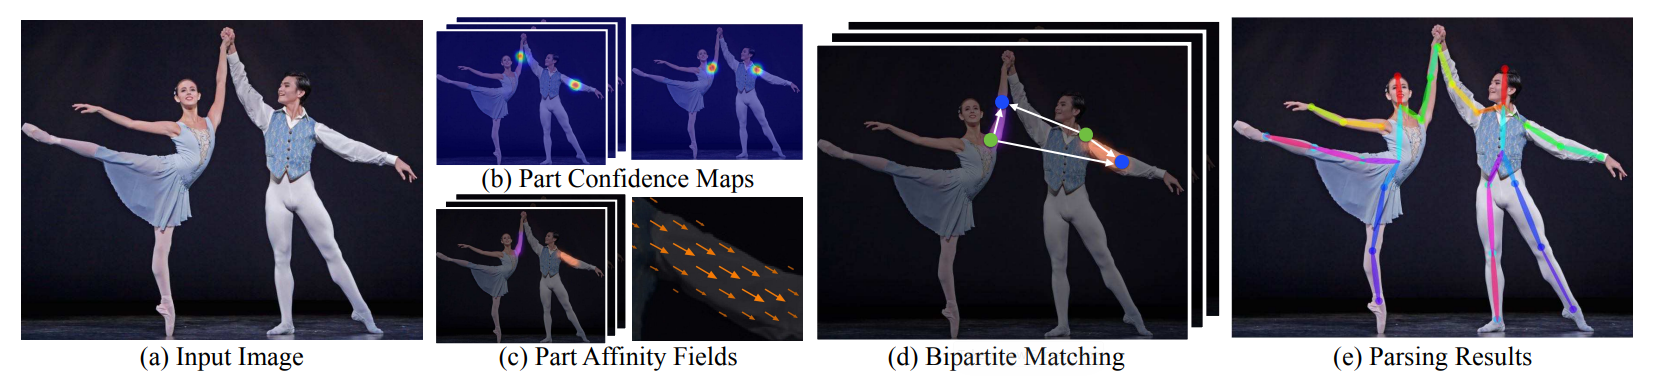
\includegraphics[width=0.8 \textwidth]{Chapters/1. HPE_LUNG/figures/openpose.png}
    \caption{OpenPose: Trabaja bajo un marco Bottom-Pp. Primero predice los mapas de confianza para
             cada parte del cuerpo $b)$ y codifican la orientación y ubicación de las extremidades
             a través $b)$ y $c)$ y finalmente asocian cada miembro identificado y reconstruyen la
             pose del cuerpo $d)$ y $e)$ \cite{8765346}.}
    \label{fig:Openpose}
\end{figure}

Top-Down: El procesamiento se realiza primero detectando los personas individualmente en la imagen
usando un bounding-box proporcionado por algun detector de objetos
\cite{DBLP:journals/corr/NewellYD16} \cite{DBLP:journals/corr/WeiRKS16},
véase la figura \ref{fig:alphapose}.
El principal problema de este enfoque es que si la detección de la persona falla ya no hay nada más
que hacer, y el costo computacional depende de la cantidad de personas en la imagen, puesto que para
cada persona detectada es necesario correr un estimador de pose entrenado para detectar una sola
persona. En contraparte a Openpose, Alpha-Pose \cite{DBLP:journals/corr/FangXL16} sigue el un marco
top-down a través de 3 componentes esenciales; \textit{Symmetric Spatial Transformer Network} (SSTN),
\textit{Parametric Pose Non-Maximum-Suppression}(NMS) y \textit{Pose-Guided Proposals Generator}
(PGPG) que les permiten minimizar el problema de la detección incorrecta o redundante de
bounding-boxes de las personas.

\begin{figure}[ht!]
    \centering
    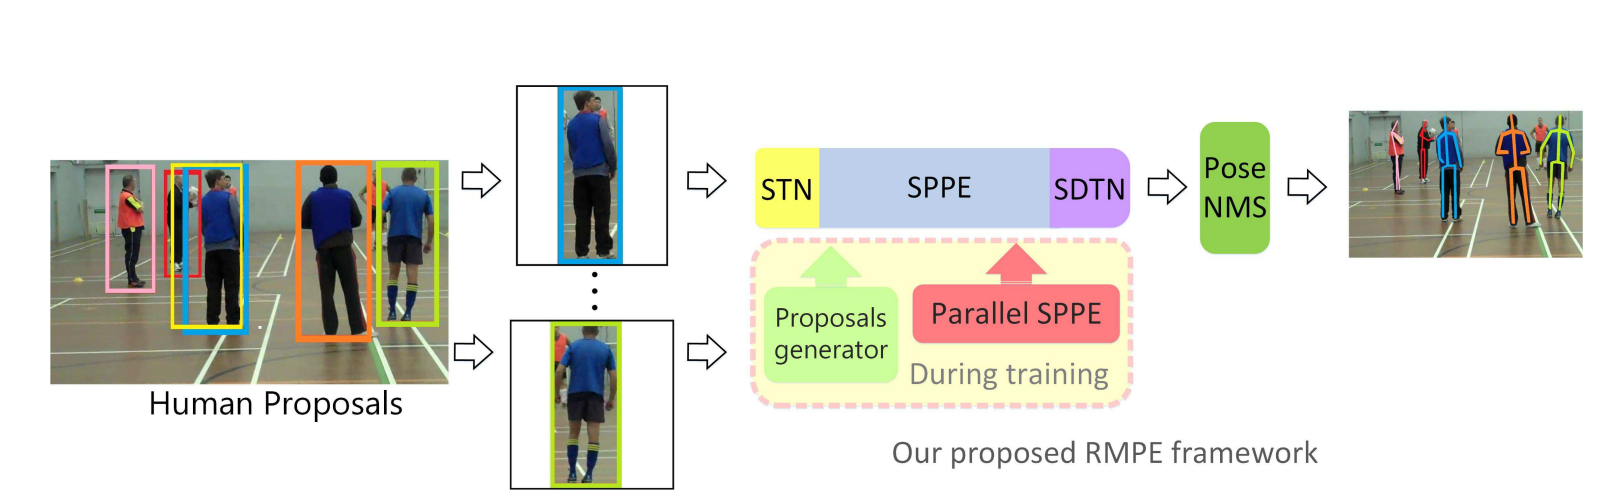
\includegraphics[width=0.8 \textwidth]{Chapters/1. HPE_LUNG/figures/alpha-pose.png}
    \caption{AlphaPose (RMPE): Trabaja bajo un marco Up-Down. Consiste en 3 principales componentes;
            El primero, \textit{Symmetric Spatial Transformer Network} (SSTN) recibe los imágenes de
            las poses a procesar y genera propuestas de poses el
            \textit{Parametric Pose Non-Maximum-Suppression}(NMS) se encarga de eliminar las
            redundancias e inconsistencias y finalmente el \textit{Pose-Guided Proposals Generator}
            (PGPG) es usado como un modelo de aumentación de datos
            \cite{DBLP:journals/corr/FangXL16}.}
    \label{fig:alphapose}
\end{figure}

La estimación de pose en 3d también puede ser realizado en dos marcos, \textit{monocular}
cuando solo se tiene una imagen de reference del sujeto de prueba en un tiempo y pose exacta
\cite{DBLP:journals/corr/MartinezHRL17} \cite{8954163} \cite{DBLP:journals/corr/abs-2002-10322}
\cite{DBLP:journals/corr/abs-1711-08585} \cite{DBLP:journals/corr/abs-2004-11822}
y multi-vista cuando se tienen imágenes desde diferentes perspectivas del sujeto de prueba en misma
la pose y tiempo exacto \cite{DBLP:journals/corr/abs-1905-05754} \cite{DBLP:journals/corr/abs-1901-04111}
\cite{DBLP:journals/corr/abs-2004-06239}.
La ventaja de usar técnicas que puedan aprovechar la información contenida
en diferentes perspectivas es que ayuda a reducir en gran medida la ambigüedad ocasionada por las
oclusiones, una parte puede no ser visible desde un ángulo pero desde otro si. Sin embargo, la
cantidad de conjunto de datos existentes para estimación de pose multi-vista es reducida.


\subsection{Modelado del Cuerpo Humano}

En la solución de los problemas de Estimación de Pose se plantea una arquitectura base para el
cuerpo humano a partir de la cual se adecuarán las estimaciones. Los modelos usados para la
representación del cuerpo humano son 3: \textit{kinematic model}, \textit{Planar Model} y
\textit{Volumetric Model}. véase la figura \ref{fig:body_model}

\begin{figure}[ht!]
    \centering
    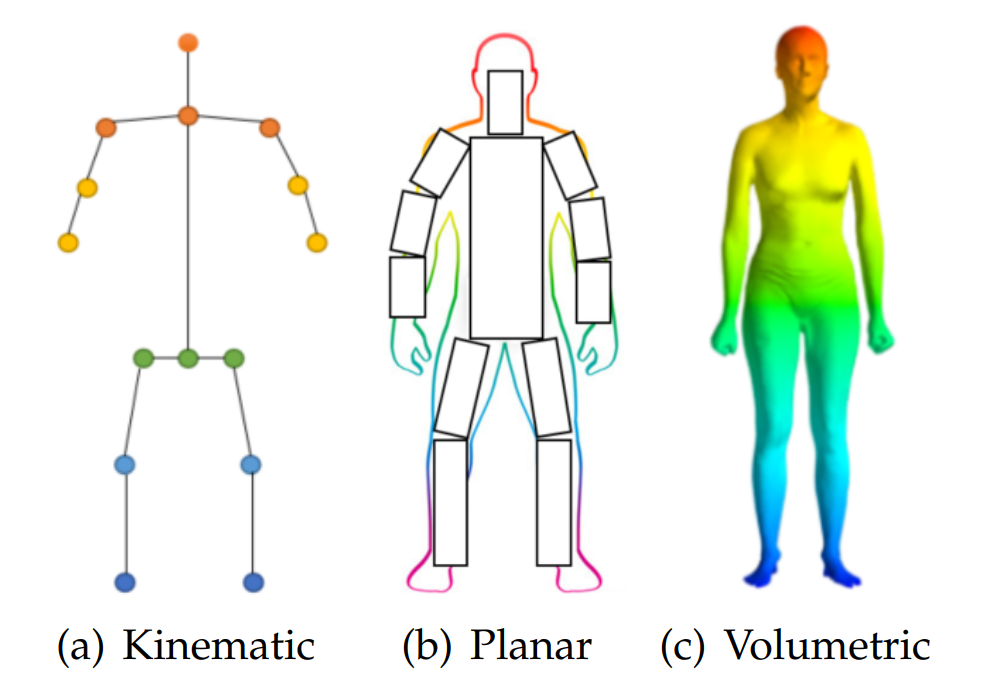
\includegraphics[width=0.7 \textwidth]{Chapters/1. HPE_LUNG/figures/body_model.png}
    \caption{Representaciones de la arquitectura del cuerpo humano. Imagen obtenida de \citeauthor{DBLP:journals/corr/FangXL16}}
    \label{fig:body_model}
\end{figure}


Skeleton base model, stick figure o kinematic model:
Es uno de los modelos más simples y mayormente usados. Consiste en grafo de nodos que representan
las articulaciones del cuerpo humano, comúnmente entre 10 y 30 nodos \cite{Felzenszwalb2005}.
Así, un hueso es representado como una conexión entre dos articulaciones. Al ser solo una
representación de la estructura del cuerpo carece de demás información como texturas o formas.

Contour-base model o Planar Model:
Es uno de los primeros modelos usados para problemas de Estimación de Pose. Los miembros y torso del
cuerpo humano son representados como un conjunto de rectángulos que proveen información tanto de los
límites de cada miembros como sus longitudes y anchor \cite{557241} \cite{COOTES199538}.

Volumen base model:
Es usado para representar el cuerpo humano y su volumen, es decir es una representación 3D del
cuerpo conseguida a través de un mallado de figuras geométricas y capturados por escaner 3D
\cite{840661}.

\subsection{Tipos de datos}

En los últimos años, debido a la masificación
de dispositivos inteligentes, el acceso a una cámara digital no resulta un problema mayor para la muchas
de las personas, así, la mayoría de los trabajos realizados sobre Estimación de Pose usan
\textit{Imágenes RGB} gracias a su fácil captura y acceso.
Sin embargo, esto solo es cierto en el contexto de la Estimación de Pose 2D, puesto que el etiquetado de datos
usando las coordenadas de la imagen como referencia no representa demasiado problema. En la
Estimación de Pose 3D, la complejidad de la obtención de los datos se incrementa. Para llevar a cabo
el proceso de obtención de los datos es necesario usar equipo especializado y costoso para la captura
de movimiento en acompañamiento de las cámaras de video \cite{6682899}. Hay dos mecanismos de captura
de movimiento, los ópticos y los no ópticos. Generalmente, en los primeros el sujeto de prueba no
necesita de aditamentos complejos como el uso de trajes
(exoesqueleto) y solo un software con ayuda de cámaras, sensores y marcadores se
encargan de registrar e interpretar el movimiento a un modelo digital. Si bien
aventajan en una reducción de coste su precisión es menor que los no ópticos.
El \textit{Kinect}, fabricado por \textit{Microsoft} es uno de los dispositivos más usados
para generar imágenes de infrarrojos (\textit{IR-image}) siendo de fácil encontrarlo y adquirirlo
gracias a su bajo conste. \cite{6165146} \cite{Izadi11kinectfusion:real-time}.

Por otra parte, existen dispositivos basados en tecnologías como \textit{LIDAR} cuya función es
generar imágenes de profundad. Al igual que el \textit{Kinect}, cada vez son de más fácil acceso
debido a su comercialización en dispositivos inteligentes en el último año por compañías como Apple
\cite{DBLP:journals/corr/abs-1711-06396}. El segundo tipo se puede dividir en dos clases;
los mecánicos los cuales usan giroscopios y acelerómetros para registrar el
movimiento y los electromagnéticos, cuyo funcionamiento es a través de la generación un campo
electromagnético y para posteriormente capturar las alteraciones en este que realiza el sujeto al
moverse \cite{articleMotion}.

\subsubsection{Conjuntos de Datos más usados para estimación de pose 2D y 3D}

\textbf{MPII Human Pose Dataset}: Es un dataset para estimación de pose en modalidades de
single-person o multi-person en 2 dimensiones \cite{andriluka14cvpr}. Incluye al rededor de 25 mil
imágenes conteniendo
40 mil de ellas de personas con anotaciones de las articulaciones del cuerpo realizando diversas
actividades. En total se agrupan en en 410 actividades recolectadas de videos de \textit{YouTube}.

\textbf{Microsoft COCO Dataset}: Es un dataset publicado por \textit{Microsoft} para tareas de
detección de objetos, segmentación y subtitulado de imágenes (image captioning), su última version
disponible corresponde a la del año 2017 \cite{DBLP:journals/corr/LinMBHPRDZ14}. Contiene al rededor
de 80 categorías de imágenes y de estas 66,808 mil son de personas con un aproximado de 250 mil
con total de aproximado de 273,469 anotaciones de cuerpos humanos. Sin embargo, No todas las
imágenes contienen anotaciones de las 17 articulaciones, por lo que los modelos tienen que predecir
cuales y cuántas articulaciones están presentes. Ambas modalidades single-person y multi-person en 2
dimensiones están disponibles en las imágenes.

% DensePose
% Number of images: 50K
% Number of annotated correspondences: 5M
% Year: 2018
% DensePose is a large-scale ground-truth dataset with image-to-surface correspondences manually
% annotated on 50K COCO images. To build this dataset Facebook AI Research team involved human
% annotators, who were establishing dense correspondences from 2D images to surface-based
% representations of the human body using a specifically developed annotation pipeline.


\textbf{HumanEva Dataset}: Dataset usado para estimación de pose en 3 dimensiones en modalidad de
single-person. Contiene diversos secuencias de videos grabadas con cámaras en formato RGB y escala
de grises. Está compuesto de dos sub-datasets \textit{HumanEva I} y \textit{HumanEva II} la principal
diferencia es el sistema de captura, el primero fue a través de software marcadores con 6 cámaras
y el segundo a través de hardware con 8 cámaras, ambos dentro de un ambiente controlado.

\textbf{Human3.6M Dataset}: Contiene aproximadamente 3.6 millones de imágenes de poses humanas
correspondientes a la cantidad de frames de secuencias de videos sobre 11 diferentes actores, 6
hombres y 3 mujeres realizando
17 distintas actividades \cite{6682899}. Cada video fue realizado a usando un total de 10 cámaras de
motion capture en un ambiente controlado interno.

\textbf{TotalCapture Dataset}: Similar a Human3.6M, contiene contiene aproximadamente 1.9 millones
de frames en videos en modalidad single-person y multi-vista calibrado a través de 8 cámaras.

\subsubsection{Conjuntos de Datos Sinteticos}

\textbf{SURREAL (Synthetic hUmans foR REAL tasks)} (2017): Es un dataset en modalidad single-person para
estimación de pose 2D y 3D. Los datos originales son tomados del dataset Human3.6M y aleatoreamente
muestreados (pose de la persona, apariencia, luz ambiental, posición de la cámara, tipos de fondos
en las imágenes, texturas, etc.) para crear sintéticamente personas y escenas
\cite{DBLP:journals/corr/Varol0MMBLS17}.

\textbf{JTA Dataset} (2018): Dataset sumamente grande creado a partir de simulaciones de
\textit{Grand Theft Auto V} desarrollado por \textit{Rockstar North} \cite{fabbri2018learning}
para estimación de poses 2D y 3D. Contiene al
rededor de 500 mil frames y 10 millones de poses de poses en escenarios urbanos todos ellos con
anotaciones completas de posiciones en 3D.

A pesar de que los datasets sintéticos son mucho grandes que los otros, actualmente no son tan
aceptados en la comunidad y su uso benchmark como benchmark no es visto principalmente dado que son
datos sinteticos. Sin embargo puesto que en los datos sintéticos se tiene mucho mayor control
del ambiente puede solventar varias de las debilidades de los otros datasets como oclusiones, cambios
de luz, tipos y colores de ropa, distintos contextos de fondos de imagen llevando modelos más robustos
y con mejor generalización. La mayoría de la bases de datos son obtenidas a través de algunos pocos
sujetos de prueba y la estructura fisiológica de individuos no es perfecta. Esta variación es causada
por diversos diversos factores como el sexo, la raza, edad, lugar de nacimiento y desarrollo,
enfermedades, factores genéticos, entre otros, además de que los movimientos recreados entre sujetos
no siempre son hechos de la misma manera aunque las circunstancias o ambiente esté controlado.

Con los datos son obtenidos bajo un ambiente controlado es posible obtener imágenes fieles para el
entrenamiento. Aún así, los modelos al ser desplegados en ambientes reales
se enfrentan a imprevistos de los que no se puede tener control; oclusiones de diversas partes del
cuerpo que no fueron provistas durante el entrenamiento ya sea por el mismo sujeto o algún objeto
extraño en la captura, movimientos extraños o rápidos como correr o dar una patada donde el modelo
no puede los puede identificar o el equipo de captura no pueda obtener que se ven como fotogramas
borrosos.

% Modern pose estimation algorithms are almost exclusively based on convolutional neural networks
% with hourglass architecture or its variants (see the image below). Such a network consists of two
% major parts: a convolutional encoder that compresses the input image into the so-called latent
% representation and decoder that constructs N heatmaps from the latent representation where N is the
% number of searched keypoints.

\subsubsection{Métricas de Evaluación}

\textbf{Percentage of Correct Parts (PCP)}: Mide la tasa de detección de extremidades. Una extremidad
o parte de un cuerpo es considerada detectada si el promedio de la distancia de las posiciones entre dos
articulaciones predichas y la distancia de las posiciones de las articulaciones de la extremidad real
es menor que cierto umbral \cite{4587468}. El umbral comúnmente tomado corresponde al 50\% de la distancia de la
longitud de la extremidad real en cuestion:

\begin{equation}
    \frac{||c_s^{(n)} - \hat{c}_s^{(n)}|| + ||c_e^{(n)} - \hat{c}_e^{(n)}||}{2} \le \alpha\ || c_s^{(n)} - c_e^{(n)} ||
    \label{eq:PCP}
\end{equation}

$||c_s^{(n)}$ y $||c_e^{(n)}$ representan las coordenadas de las dos articulaciones (inicial y final
respectivamente) de la n-ésima extremidad. $||\hat c_s^{(n)}$ y $||\hat c_e^{(n)}$ son las coordenadas
inicial y final de las dos articulaciones predichas de la n-ésima extremidad. $\alpha$ funciona como
el umbral de error. Actualmente, ya no se usa esta métrica debido a que penaliza mayormente las partes
del cuerpo más pequeñas. Mientras mayor es su \textit{PCP} mejor es el modelo.


\textbf{Percentage of Detected Joints (PDJ)}: Esta métrica fue propuesta para sobrellevar la
limitante antes mencionada de \textit{PCP}. Mide la tasa de detección de articulaciones del cuerpo.
Una articulación es correctamente detectada si la distancia entre la posición de la articulación
detectada y la posición real de la articulación está dentro de cierta fracción del diámetro del torso,
es decir la distancia entre la cadera derecha (right hip) y el hombro izquierdo (left shoulder)
\cite{6619315} \cite{DBLP:journals/corr/ToshevS13}:

\begin{equation}
    ||c^{(i)} - \hat{c}^{(i)}|| \le \alpha\ || c_{rh} - c_{ls} ||
    \label{eq:PDJ}
\end{equation}

$c^{(i)}$ es la coordenada de la i-ésima articulación y $\hat c^{(i)}$ es la coordenada de la
articulación predicha correspondiente. $c_{rh}$ es la coordenada de la cadera derecha y $c_{ls}$
es la coordenada del hombro izquierdo. El problema con esta métrica es que cuando la persona se es
capturada de lado en una imagen 2D el diámetro del torso tiende a ser cero así como la distancia
entre la cadera derecha e izquierda.

\textbf{Percentage of Correct Key-points (PCK)}: Es similar a la métrica \textit{PDJ} pero en vez de
tomar el diámetro del torso se toma la distancia de la diagonal del rectangulo externo que rodea
todas las articulaciones del cuerpo \cite{6380498}.

\begin{equation}
    ||c^{(i)} - \hat{c}^{(i)}|| \le \alpha\ diag_{bbox}
    \label{eq:PCK}
\end{equation}

La ecuación \ref{eq:PCK} correspondiente al cálculo de la detección correcta de articulación para la
métrica de \textit{PCK} es similar a \textit{PDJ}. Una tercer variación es considerando una
proporción de la longitud del segmente de la cabeza como umbral \cite{6909866},
\textit{head-normalized probability of the correct keypoint} o \textit{PCKh}, con la finalidad
de tener un umbral independiente de las distancias de las articulaciones y una posible elección
es usar el tamaño de la cabeza del sujeto a prueba.

\textbf{Average Precision (AP) y Average Recall (AR)}: Inicialmente introducido
como  \textit{Average Precision of Keypoints (APK)} \cite{6380498} mide la exactitud y rendimiento
de la detección de las articulaciones de acuerdo a la proporción de verdaderos positivos sobre el
total de positivos detectados (precision) $\frac{TP}{TP + FP}$ y la proporción
de verdaderos positivos sobre el total de positivos (recall) $\frac{TP}{TP + FN}$ penalizando tanto
detecciones no encontradas como falsas detecciones. Al igual que los anteriores hay variantes
como Mean Average Precision (mAP) que es la media de la precisión del modelo para todas las
clase. Todos basados en alguna medida de similaridad como la propuesta en
\textit{Object Key-points Similarity (OKS)} que mide el promedio de cercania de las articulaciones
predichas y las reales. Definen una similaridad entre articulaciones (Keypoint Similarity)
\cite{DBLP:journals/corr/LinMBHPRDZ14}
como la distancia entre las articulaciones predichas normalizadas por la escala del
área que forma la persona y una constante de regularización determinada para cada articulación:

\begin{equation}
    KS = \exp(- \frac{||c^{(n)} - \hat{c}^{(n)}||^2}{2s^2 k^2_n})
    \label{eq:KS}
\end{equation}

$s$ y $k_n$ corresponden al factor de escala equivalente a la raíz cuadrada del área segmentada del
objeto y a la constante de regularización por cada tipo de articulación cuya su función conjunta
es regular la importancia de cada articulación.


\textbf{Mean Per Joint Position Error (MPJPE)}: Calcula el error en milímetros determinado por la distancia
euclidiana entre los articulaciones predichas y las reales sobre cada tipo de articulación de la
imagen o imágenes en caso de videos. Para distintos datasets de predicción de pose en 3D existen
más de un pre-procesamiento antes calcular el error \textit{MPJPE} conocidos como protocolos.
Por ejemplo para \textit{Human3.6M} el Protocolo \#1 consiste en alinear las coordenadas de las
articulaciones con respecto a la raíz, generalmente la que corresponde al centro de la cadera (hip).
El Protocolo \#2 calcula el error después de realizar un alineamiento mediante una transformación
rígida usando \textit{Procrustes Analysis} \cite{Gower1975}, también abreviado como \textit{P-MPJPE}.

\begin{equation}
    MPJPE = \frac{1}{M} \sum_{i=1}^M ||c^{(i)} - \hat{c}^{(i)}||
    \label{eq:MPJPE}
\end{equation}

$M$ corresponde a el total de articulaciones. Generalmente el error es calculado por tipo, clase o
acción representado en los videos.

Al igual que en estimación de pose 2D la métrica de PCK o 3DPKC es usada para estimación de pose en
3D, al igual que su area bajo la Curva (AUC) considerando típicamente un umbral de 150mm que se
aproxima a la mitad del tamaño de la cabeza \cite{DBLP:journals/corr/MehtaRCSXT16}. Por otro lado,
datasets usados para estimación de pose 3D son basados en secuencias de videos y una variante a
\textit{MPJPE} es introducida \cite{8954163} para considerar la suavidad de las transiciones entre
poses midiendo la velocidad de las articulaciones (en milímetros por segundo),
\textit{Mean Per Join Velocity Error (MPJVE)}, que corresponde al error \textit{MPJPE} primer
derivada de las secuencias de pose 3D.

\textbf{Mean Joint Angle Error (MJAE)}: Es similar al error \textit{MPJPE} pero usando los ángulos de
cada articulación. Mide el error como promedio sobre todos los ángulos de la diferencia absoluta
entre la articulación estimada y la real de acuerdo a su posición angular:

\begin{equation}
    MPJPE = \frac{1}{M} \sum_{i=1}^M |(c^{(i)} - \hat{c}^{(i)}) \mod \pm 180^{\circ}|
    \label{eq:MJAE}
\end{equation}
